\documentclass[aspectratio=169]{beamer}

% ── Theme ────────────────────────────────────────────────────────────────────
\usetheme{metropolis}
\usepackage{appendixnumberbeamer}
\usepackage{booktabs}
\usepackage{graphicx}
\usepackage{tikz}
\usetikzlibrary{arrows.meta, positioning, shapes, shapes.geometric}
\usepackage{fontawesome5}
\usepackage{xcolor}

% ── Blue colour palette ───────────────────────────────────────────────────────
\definecolor{primary}{HTML}{1d4ed8}      % deep blue
\definecolor{accent}{HTML}{3b82f6}       % mid blue
\definecolor{lightblue}{HTML}{dbeafe}    % very light blue
\definecolor{darkblue}{HTML}{1e3a8a}     % navy
\definecolor{slategray}{HTML}{475569}
\definecolor{lightgray}{HTML}{f8fafc}

\setbeamercolor{normal text}{fg=darkblue}
\setbeamercolor{frametitle}{bg=primary, fg=white}
\setbeamercolor{progress bar}{fg=accent}
\setbeamercolor{alerted text}{fg=accent}
\setbeamercolor{title separator}{fg=accent}
\setbeamercolor{block title}{bg=lightblue, fg=darkblue}

% ── Meta ─────────────────────────────────────────────────────────────────────
\title{\textbf{News \& Context Explainer}}
\subtitle{An LLM Agent Built from Scratch}
\author{Yue Wu}
\date{}

% ─────────────────────────────────────────────────────────────────────────────
\begin{document}

\maketitle

% ── 1. The Problem ────────────────────────────────────────────────────────────
\begin{frame}{The Problem}
  \begin{columns}[T]
    \begin{column}{0.55\textwidth}
      \vspace{0.4cm}
      You read a headline.\\[0.6em]
      \textit{``US imposes 145\% tariffs on Chinese goods''}\\[0.8em]
      But you don't know:
      \begin{itemize}
        \item What triggered this?
        \item How did US-China trade get here?
        \item What does 145\% actually cost in dollars?
      \end{itemize}
      \vspace{0.6em}
      You open 5 tabs, skim Wikipedia, do some math\ldots\\
      \textbf{20 minutes later, you kind of get it.}
    \end{column}
    \begin{column}{0.4\textwidth}
      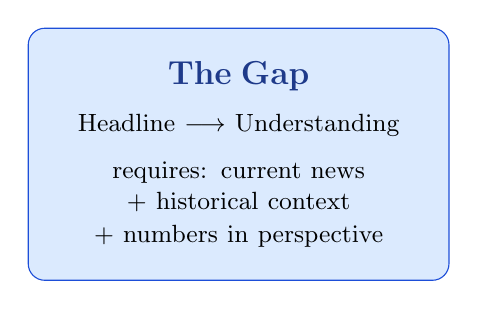
\begin{tikzpicture}
        \node[draw=primary, fill=lightblue, rounded corners=6pt,
              text width=4.5cm, align=center, inner sep=12pt] {
          \textcolor{darkblue}{\textbf{\large The Gap}}\\[6pt]
          \small Headline $\longrightarrow$ Understanding\\[6pt]
          \small requires: current news\\
          + historical context\\
          + numbers in perspective
        };
      \end{tikzpicture}
    \end{column}
  \end{columns}
\end{frame}

% ── 2. Plain LLM vs Agent ────────────────────────────────────────────────────
\begin{frame}{Why Not Just Ask ChatGPT?}
  \begin{columns}[T]
    \begin{column}{0.47\textwidth}
      \textcolor{darkblue}{\textbf{Plain LLM}}\\[0.5em]
      \begin{itemize}
        \setlength\itemsep{0.4em}
        \item[\textcolor{red}{$\times$}] \textbf{Hallucination} — confidently states\\
              wrong facts with no source
        \item[\textcolor{red}{$\times$}] \textbf{Knowledge cutoff} — unaware of\\
              anything after training date
        \item[\textcolor{red}{$\times$}] \textbf{No calculation} — makes arithmetic\\
              errors on multi-step math
        \item[\textcolor{red}{$\times$}] \textbf{No citations} — no way to verify\\
              where the answer came from
        \item[\textcolor{red}{$\times$}] \textbf{Static} — same answer every time,\\
              regardless of current events
      \end{itemize}
    \end{column}
    \hfill
    \begin{column}{0.47\textwidth}
      \textcolor{primary}{\textbf{LLM Agent (ours)}}\\[0.5em]
      \begin{itemize}
        \setlength\itemsep{0.4em}
        \item[\textcolor{primary}{$\checkmark$}] \textbf{Grounded} — answers backed by\\
              real web pages \& Wikipedia
        \item[\textcolor{primary}{$\checkmark$}] \textbf{Up-to-date} — searches the web\\
              for today's information
        \item[\textcolor{primary}{$\checkmark$}] \textbf{Exact math} — delegates numbers\\
              to a safe calculator tool
        \item[\textcolor{primary}{$\checkmark$}] \textbf{Cited} — every fact has a\\
              traceable source URL
        \item[\textcolor{primary}{$\checkmark$}] \textbf{Adaptive} — plans which tools\\
              to use based on the question
      \end{itemize}
    \end{column}
  \end{columns}
  \vspace{0.5em}
  \begin{center}
    \small\textit{Our TriviaQA eval confirms this: agent 83\% vs.\ plain LLM 77\%}
  \end{center}
\end{frame}

% ── 3. Solution ───────────────────────────────────────────────────────────────
\begin{frame}{The Solution}
  \begin{center}
    {\Large \textbf{News \& Context Explainer}}\\[0.5em]
    {\large An autonomous LLM agent that bridges the gap}
  \end{center}
  \vspace{0.4cm}
  \begin{columns}[T]
    \begin{column}{0.32\textwidth}
      \centering
      \textcolor{primary}{\Large \faSearch}\\[4pt]
      \textbf{Current News}\\[4pt]
      \small What's happening right now
    \end{column}
    \begin{column}{0.32\textwidth}
      \centering
      \textcolor{primary}{\Large \faBook}\\[4pt]
      \textbf{Historical Context}\\[4pt]
      \small How we got here, key players
    \end{column}
    \begin{column}{0.32\textwidth}
      \centering
      \textcolor{primary}{\Large \faCalculator}\\[4pt]
      \textbf{Numbers in Perspective}\\[4pt]
      \small What the figures actually mean
    \end{column}
  \end{columns}
  \vspace{0.6cm}
  \begin{center}
    \textit{One question in. One complete answer out.}
  \end{center}
\end{frame}

% ── 3. The Three Tools ────────────────────────────────────────────────────────
\begin{frame}{Three Tools, One Purpose}
  \begin{table}
    \begin{tabular}{lll}
      \toprule
      \textbf{Tool} & \textbf{Source} & \textbf{Role} \\
      \midrule
      \texttt{web\_search} & Tavily Search API & Real-time news, published dates \\[4pt]
      \texttt{wikipedia\_lookup} & Wikipedia REST API & Historical background \& context \\[4pt]
      \texttt{calculator} & Python AST (safe eval) & Tariffs, GDP ratios, percentages \\
      \bottomrule
    \end{tabular}
  \end{table}
  \vspace{0.4cm}
  \textbf{Example — US-China Trade War:}
  \begin{enumerate}
      \item \texttt{web\_search("US China tariffs 2026")} $\rightarrow$ latest headlines
    \item \texttt{wikipedia\_lookup("China–United States trade war")} $\rightarrow$ history
    \item \texttt{calculator("500000000000 * 0.145")} $\rightarrow$ \$72.5B cost
  \end{enumerate}
\end{frame}

% ── 4. Agent Architecture ─────────────────────────────────────────────────────
\begin{frame}{Agent Architecture — ReAct Loop}
  \begin{center}
  \begin{tikzpicture}[
    node distance=1.1cm,
    box/.style={draw=primary, rounded corners=4pt, fill=primary, text=white,
                minimum width=2.6cm, minimum height=0.72cm,
                font=\small\bfseries, align=center},
    tool/.style={draw=accent, rounded corners=4pt, fill=lightblue,
                 text=darkblue, minimum width=2.6cm, minimum height=0.6cm,
                 font=\footnotesize\bfseries, align=center},
    arr/.style={-{Stealth}, thick, color=accent}
  ]
    \node[box] (user)  {User Query};
    \node[box, right=1.3cm of user]  (think) {Think\\{\tiny LLM reasons}};
    \node[box, right=1.3cm of think] (act)   {Act\\{\tiny Call tool}};
    \node[box, right=1.3cm of act]   (obs)   {Observe\\{\tiny Feed result back}};
    \node[box, below=1.1cm of act]   (ans)   {Final Answer};
    \node[tool, below=0.45cm of think] (tools)
          {\textcolor{primary}{\faSearch}\ \textcolor{primary}{\faBook}\ \textcolor{primary}{\faCalculator}};

    \draw[arr] (user)  -- (think);
    \draw[arr] (think) -- (act);
    \draw[arr] (act)   -- (obs);
    \draw[arr] (obs)   to[bend left=40]
               node[above, font=\tiny, color=slategray]{repeat} (think);
    \draw[arr] (act)   -- (ans)
               node[midway, right, font=\tiny, color=slategray]{no tool call};
    \draw[arr, dashed, color=accent!60] (act) -- (tools);
  \end{tikzpicture}
  \end{center}
  \vspace{0.2cm}
  \begin{columns}
    \begin{column}{0.5\textwidth}
      \begin{itemize}
        \item Written \textbf{from scratch} — no LangChain, no CrewAI
        \item Max 10 iterations (loop guard)
      \end{itemize}
    \end{column}
    \begin{column}{0.5\textwidth}
      \begin{itemize}
        \item \textbf{LLM:} Qwen3-32B via Groq (free tier)
        \item Tool schemas in OpenAI JSON format
      \end{itemize}
    \end{column}
  \end{columns}
\end{frame}

% ── 5. Design Choices ─────────────────────────────────────────────────────────
\begin{frame}{Key Design Choices}
  \begin{table}
    \begin{tabular}{ll}
      \toprule
      \textbf{Decision} & \textbf{Rationale} \\
      \midrule
      Groq + Qwen3-32B & Free tier, fast inference, strong tool calling \\[4pt]
      Tavily Search API & Purpose-built for LLM agents, real-time results \\[4pt]
      OpenAI-compatible API & Keeps tool schemas provider-agnostic \\[4pt]
      Wikipedia REST API & Structured, reliable, always available \\[4pt]
      Safe AST calculator & No \texttt{eval()} security risk \\[4pt]
      Gradio 6 UI & Minimal setup, collapsible tool traces \\
      \bottomrule
    \end{tabular}
  \end{table}
\end{frame}

% ── 6. Interface ──────────────────────────────────────────────────────────────
\begin{frame}{User Interface}
  \begin{columns}[T]
    \begin{column}{0.5\textwidth}
      \vspace{0.3cm}
      Built with \textbf{Gradio 6}:
      \begin{itemize}
        \item Chat-style bubble layout
        \item Example news prompts to click
        \item \textbf{Collapsible tool traces}\\
              {\small \textcolor{primary}{\faSearch\ \faBook\ \faCalculator}\ show reasoning steps}
        \item Clear conversation button
        \item Runs locally at \texttt{localhost:7860}
      \end{itemize}
      \vspace{0.4cm}
      \textit{[Live demo here]}
    \end{column}
    \begin{column}{0.45\textwidth}
      \begin{tikzpicture}
        \node[draw=primary, rounded corners=6pt, fill=lightgray,
              text width=5.2cm, inner sep=10pt] {
          \footnotesize
          \textcolor{darkblue}{\textbf{\faNewspaper\ News \& Context Explainer}}\\[4pt]
          \rule{\linewidth}{0.4pt}\\[4pt]
          \textit{User:} What's happening with\\
          the US-China trade war?\\[4pt]
          \rule{\linewidth}{0.2pt}\\[3pt]
          \textcolor{accent}{$\triangleright$ \faSearch\ web\_search(\ldots)}\\
          \textcolor{accent}{$\triangleright$ \faBook\ wikipedia\_lookup(\ldots)}\\
          \textcolor{accent}{$\triangleright$ \faCalculator\ calculator(\ldots)}\\[4pt]
          \rule{\linewidth}{0.2pt}\\[3pt]
          \textit{Agent:} The US-China trade war\ldots
        };
      \end{tikzpicture}
    \end{column}
  \end{columns}
\end{frame}

% ── 7. Evaluation ─────────────────────────────────────────────────────────────
\begin{frame}{Evaluation — Agent vs.\ Plain LLM}
  \begin{columns}[T]
    \begin{column}{0.48\textwidth}
      \vspace{0.3cm}
      \textbf{Setup}
      \begin{itemize}
        \item Dataset: \textbf{TriviaQA} (public, HuggingFace)
        \item 100 validation questions
        \item Each question run \textbf{twice}:\\
              with tools vs.\ without tools
        \item Scoring: answer-in-prediction\\
              {\small (standard TriviaQA metric)}
      \end{itemize}
      \vspace{0.4cm}
      \large \textbf{Result: \textcolor{primary}{+6\% improvement}}\\[4pt]
      \small Avg 1.0 tool calls/question\\
      0 crashes across 100 runs
    \end{column}
    \begin{column}{0.48\textwidth}
      \centering
      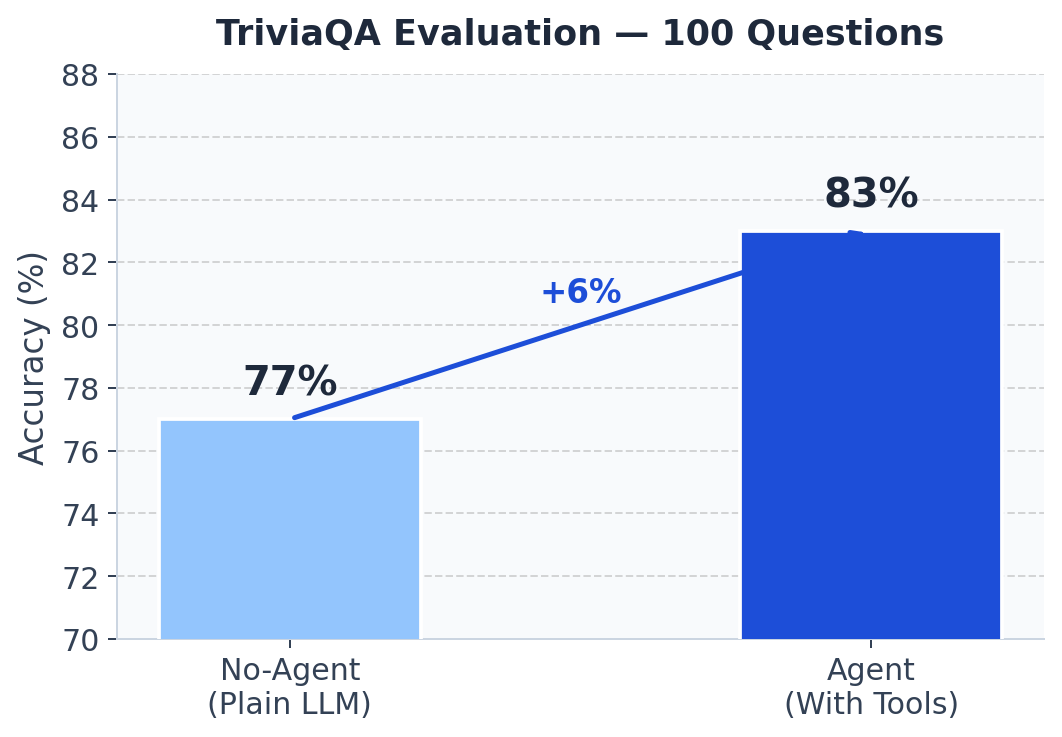
\includegraphics[width=\linewidth]{eval_chart.png}
    \end{column}
  \end{columns}
\end{frame}

% ── 8. Summary ────────────────────────────────────────────────────────────────
\begin{frame}{Summary}
  \begin{columns}[T]
    \begin{column}{0.5\textwidth}
      \vspace{0.3cm}
      \textbf{What was built:}
      \begin{itemize}
        \item ReAct agent loop from scratch
        \item 3 tools: search, Wikipedia, calculator
        \item Gradio chat UI with tool traces
        \item Evaluation on TriviaQA (100 Qs)
      \end{itemize}
      \vspace{0.5cm}
      \textbf{Key result:}\\
      Agent outperforms bare LLM by \alert{+6\%}\\
      on a real public benchmark
    \end{column}
    \begin{column}{0.45\textwidth}
      \vspace{0.3cm}
      \textbf{GitHub:}\\[4pt]
      \small \texttt{github.com/202520030411/}\\
      \texttt{LLM\_agent\_from\_scratch}\\[1cm]
      \textbf{Stack:}\\[4pt]
      Python $\cdot$ Groq $\cdot$ Qwen3-32B\\
      Gradio $\cdot$ Tavily $\cdot$ Wikipedia
    \end{column}
  \end{columns}
\end{frame}

\end{document}
